\documentclass[1p]{elsarticle_modified}
%\bibliographystyle{elsarticle-num}

%\usepackage[colorlinks]{hyperref}
%\usepackage{abbrmath_seonhwa} %\Abb, \Ascr, \Acal ,\Abf, \Afrak
\usepackage{amsfonts}
\usepackage{amssymb}
\usepackage{amsmath}
\usepackage{amsthm}
\usepackage{scalefnt}
\usepackage{amsbsy}
\usepackage{kotex}
\usepackage{caption}
\usepackage{subfig}
\usepackage{color}
\usepackage{graphicx}
\usepackage{xcolor} %% white, black, red, green, blue, cyan, magenta, yellow
\usepackage{float}
\usepackage{setspace}
\usepackage{hyperref}

\usepackage{tikz}
\usetikzlibrary{arrows}

\usepackage{multirow}
\usepackage{array} % fixed length table
\usepackage{hhline}

%%%%%%%%%%%%%%%%%%%%%
\makeatletter
\renewcommand*\env@matrix[1][\arraystretch]{%
	\edef\arraystretch{#1}%
	\hskip -\arraycolsep
	\let\@ifnextchar\new@ifnextchar
	\array{*\c@MaxMatrixCols c}}
\makeatother %https://tex.stackexchange.com/questions/14071/how-can-i-increase-the-line-spacing-in-a-matrix
%%%%%%%%%%%%%%%

\usepackage[normalem]{ulem}

\newcommand{\msout}[1]{\ifmmode\text{\sout{\ensuremath{#1}}}\else\sout{#1}\fi}
%SOURCE: \msout is \stkout macro in https://tex.stackexchange.com/questions/20609/strikeout-in-math-mode

\newcommand{\cancel}[1]{
	\ifmmode
	{\color{red}\msout{#1}}
	\else
	{\color{red}\sout{#1}}
	\fi
}

\newcommand{\add}[1]{
	{\color{blue}\uwave{#1}}
}

\newcommand{\replace}[2]{
	\ifmmode
	{\color{red}\msout{#1}}{\color{blue}\uwave{#2}}
	\else
	{\color{red}\sout{#1}}{\color{blue}\uwave{#2}}
	\fi
}

\newcommand{\Sol}{\mathcal{S}} %segment
\newcommand{\D}{D} %diagram
\newcommand{\A}{\mathcal{A}} %arc


%%%%%%%%%%%%%%%%%%%%%%%%%%%%%5 test

\def\sl{\operatorname{\textup{SL}}(2,\Cbb)}
\def\psl{\operatorname{\textup{PSL}}(2,\Cbb)}
\def\quan{\mkern 1mu \triangleright \mkern 1mu}

\theoremstyle{definition}
\newtheorem{thm}{Theorem}[section]
\newtheorem{prop}[thm]{Proposition}
\newtheorem{lem}[thm]{Lemma}
\newtheorem{ques}[thm]{Question}
\newtheorem{cor}[thm]{Corollary}
\newtheorem{defn}[thm]{Definition}
\newtheorem{exam}[thm]{Example}
\newtheorem{rmk}[thm]{Remark}
\newtheorem{alg}[thm]{Algorithm}

\newcommand{\I}{\sqrt{-1}}
\begin{document}

%\begin{frontmatter}
%
%\title{Boundary parabolic representations of knots up to 8 crossings}
%
%%% Group authors per affiliation:
%\author{Yunhi Cho} 
%\address{Department of Mathematics, University of Seoul, Seoul, Korea}
%\ead{yhcho@uos.ac.kr}
%
%
%\author{Seonhwa Kim} %\fnref{s_kim}}
%\address{Center for Geometry and Physics, Institute for Basic Science, Pohang, 37673, Korea}
%\ead{ryeona17@ibs.re.kr}
%
%\author{Hyuk Kim}
%\address{Department of Mathematical Sciences, Seoul National University, Seoul 08826, Korea}
%\ead{hyukkim@snu.ac.kr}
%
%\author{Seokbeom Yoon}
%\address{Department of Mathematical Sciences, Seoul National University, Seoul, 08826,  Korea}
%\ead{sbyoon15@snu.ac.kr}
%
%\begin{abstract}
%We find all boundary parabolic representation of knots up to 8 crossings.
%
%\end{abstract}
%\begin{keyword}
%    \MSC[2010] 57M25 
%\end{keyword}
%
%\end{frontmatter}

%\linenumbers
%\tableofcontents
%
\newcommand\colored[1]{\textcolor{white}{\rule[-0.35ex]{0.8em}{1.4ex}}\kern-0.8em\color{red} #1}%
%\newcommand\colored[1]{\textcolor{white}{ #1}\kern-2.17ex	\textcolor{white}{ #1}\kern-1.81ex	\textcolor{white}{ #1}\kern-2.15ex\color{red}#1	}

{\Large $\underline{12a_{0329}~(K12a_{0329})}$}

\setlength{\tabcolsep}{10pt}
\renewcommand{\arraystretch}{1.6}
\vspace{1cm}\begin{tabular}{m{100pt}>{\centering\arraybackslash}m{274pt}}
\multirow{5}{120pt}{
	\centering
	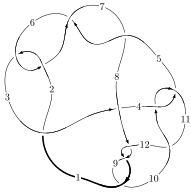
\includegraphics[width=112pt]{../../../GIT/diagram.site/Diagrams/png/1130_12a_0329.png}\\
\ \ \ A knot diagram\footnotemark}&
\allowdisplaybreaks
\textbf{Linearized knot diagam} \\
\cline{2-2}
 &
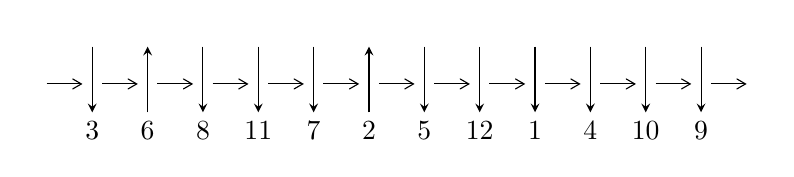
\begin{tikzpicture}[x=20pt, y=17pt]
	% nodes
	\node (C0) at (0, 0) {};
	\node (C1) at (1, 0) {};
	\node (C1U) at (1, +1) {};
	\node (C1D) at (1, -1) {3};

	\node (C2) at (2, 0) {};
	\node (C2U) at (2, +1) {};
	\node (C2D) at (2, -1) {6};

	\node (C3) at (3, 0) {};
	\node (C3U) at (3, +1) {};
	\node (C3D) at (3, -1) {8};

	\node (C4) at (4, 0) {};
	\node (C4U) at (4, +1) {};
	\node (C4D) at (4, -1) {11};

	\node (C5) at (5, 0) {};
	\node (C5U) at (5, +1) {};
	\node (C5D) at (5, -1) {7};

	\node (C6) at (6, 0) {};
	\node (C6U) at (6, +1) {};
	\node (C6D) at (6, -1) {2};

	\node (C7) at (7, 0) {};
	\node (C7U) at (7, +1) {};
	\node (C7D) at (7, -1) {5};

	\node (C8) at (8, 0) {};
	\node (C8U) at (8, +1) {};
	\node (C8D) at (8, -1) {12};

	\node (C9) at (9, 0) {};
	\node (C9U) at (9, +1) {};
	\node (C9D) at (9, -1) {1};

	\node (C10) at (10, 0) {};
	\node (C10U) at (10, +1) {};
	\node (C10D) at (10, -1) {4};

	\node (C11) at (11, 0) {};
	\node (C11U) at (11, +1) {};
	\node (C11D) at (11, -1) {10};

	\node (C12) at (12, 0) {};
	\node (C12U) at (12, +1) {};
	\node (C12D) at (12, -1) {9};
	\node (C13) at (13, 0) {};

	% arrows
	\draw[->,>={angle 60}]
	(C0) edge (C1) (C1) edge (C2) (C2) edge (C3) (C3) edge (C4) (C4) edge (C5) (C5) edge (C6) (C6) edge (C7) (C7) edge (C8) (C8) edge (C9) (C9) edge (C10) (C10) edge (C11) (C11) edge (C12) (C12) edge (C13) ;	\draw[->,>=stealth]
	(C1U) edge (C1D) (C2D) edge (C2U) (C3U) edge (C3D) (C4U) edge (C4D) (C5U) edge (C5D) (C6D) edge (C6U) (C7U) edge (C7D) (C8U) edge (C8D) (C9U) edge (C9D) (C10U) edge (C10D) (C11U) edge (C11D) (C12U) edge (C12D) ;
	\end{tikzpicture} \\
\hhline{~~} \\& 
\textbf{Solving Sequence} \\ \cline{2-2} 
 &
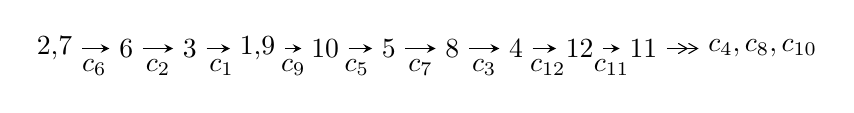
\begin{tikzpicture}[x=23pt, y=7pt]
	% node
	\node (A0) at (-1/8, 0) {2,7};
	\node (A1) at (1, 0) {6};
	\node (A2) at (2, 0) {3};
	\node (A3) at (49/16, 0) {1,9};
	\node (A4) at (33/8, 0) {10};
	\node (A5) at (41/8, 0) {5};
	\node (A6) at (49/8, 0) {8};
	\node (A7) at (57/8, 0) {4};
	\node (A8) at (65/8, 0) {12};
	\node (A9) at (73/8, 0) {11};
	\node (C1) at (1/2, -1) {$c_{6}$};
	\node (C2) at (3/2, -1) {$c_{2}$};
	\node (C3) at (5/2, -1) {$c_{1}$};
	\node (C4) at (29/8, -1) {$c_{9}$};
	\node (C5) at (37/8, -1) {$c_{5}$};
	\node (C6) at (45/8, -1) {$c_{7}$};
	\node (C7) at (53/8, -1) {$c_{3}$};
	\node (C8) at (61/8, -1) {$c_{12}$};
	\node (C9) at (69/8, -1) {$c_{11}$};
	\node (A10) at (11, 0) {$c_{4},c_{8},c_{10}$};

	% edge
	\draw[->,>=stealth]	
	(A0) edge (A1) (A1) edge (A2) (A2) edge (A3) (A3) edge (A4) (A4) edge (A5) (A5) edge (A6) (A6) edge (A7) (A7) edge (A8) (A8) edge (A9) ;
	\draw[->>,>={angle 60}]	
	(A9) edge (A10);
\end{tikzpicture} \\ 

\end{tabular} \\

\footnotetext{
The image of knot diagram is generated by the software ``\textbf{Draw programme}" developed by Andrew Bartholomew(\url{http://www.layer8.co.uk/maths/draw/index.htm\#Running-draw}), where we modified some parts for our purpose(\url{https://github.com/CATsTAILs/LinksPainter}).
}\phantom \\ \newline 
\centering \textbf{Ideals for irreducible components\footnotemark of $X_{\text{par}}$} 
 
\begin{align*}
I^u_{1}&=\langle 
u^{72}+u^{71}+\cdots+b- u,\;u^{72}+u^{71}+\cdots+a-1,\;u^{74}+2 u^{73}+\cdots-3 u+1\rangle \\
I^u_{2}&=\langle 
u^3+u^2+b,\;u^3+u^2+a+u,\;u^4+u^3+u^2+1\rangle \\
\\
\end{align*}
\raggedright * 2 irreducible components of $\dim_{\mathbb{C}}=0$, with total 78 representations.\\
\footnotetext{All coefficients of polynomials are rational numbers. But the coefficients are sometimes approximated in decimal forms when there is not enough margin.}
\newpage
\renewcommand{\arraystretch}{1}
\centering \section*{I. $I^u_{1}= \langle u^{72}+u^{71}+\cdots+b- u,\;u^{72}+u^{71}+\cdots+a-1,\;u^{74}+2 u^{73}+\cdots-3 u+1 \rangle$}
\flushleft \textbf{(i) Arc colorings}\\
\begin{tabular}{m{7pt} m{180pt} m{7pt} m{180pt} }
\flushright $a_{2}=$&$\begin{pmatrix}0\\u\end{pmatrix}$ \\
\flushright $a_{7}=$&$\begin{pmatrix}1\\0\end{pmatrix}$ \\
\flushright $a_{6}=$&$\begin{pmatrix}1\\u^2\end{pmatrix}$ \\
\flushright $a_{3}=$&$\begin{pmatrix}u\\u^3+u\end{pmatrix}$ \\
\flushright $a_{1}=$&$\begin{pmatrix}u^3\\u^5+u^3+u\end{pmatrix}$ \\
\flushright $a_{9}=$&$\begin{pmatrix}- u^{72}- u^{71}+\cdots+2 u+1\\- u^{72}- u^{71}+\cdots- u^2+u\end{pmatrix}$ \\
\flushright $a_{10}=$&$\begin{pmatrix}-2 u^{72}- u^{71}+\cdots-7 u^2+6 u\\u^{73}- u^{72}+\cdots-3 u^2+2 u\end{pmatrix}$ \\
\flushright $a_{5}=$&$\begin{pmatrix}u^2+1\\u^2\end{pmatrix}$ \\
\flushright $a_{8}=$&$\begin{pmatrix}u^4+u^2+1\\u^4\end{pmatrix}$ \\
\flushright $a_{4}=$&$\begin{pmatrix}- u^{11}-2 u^9-4 u^7-4 u^5-3 u^3\\- u^{11}- u^9-2 u^7- u^5+u^3+u\end{pmatrix}$ \\
\flushright $a_{12}=$&$\begin{pmatrix}- u^{71}- u^{70}+\cdots- u+1\\- u^{73}- u^{72}+\cdots+2 u^2+u\end{pmatrix}$ \\
\flushright $a_{11}=$&$\begin{pmatrix}- u^{71}- u^{70}+\cdots+u+1\\- u^{73}- u^{72}+\cdots+3 u^2+u\end{pmatrix}$\\&\end{tabular}
\flushleft \textbf{(ii) Obstruction class $= -1$}\\~\\
\flushleft \textbf{(iii) Cusp Shapes $= 4 u^{73}+33 u^{71}+\cdots+26 u-15$}\\~\\
\newpage\renewcommand{\arraystretch}{1}
\flushleft \textbf{(iv) u-Polynomials at the component}\newline \\
\begin{tabular}{m{50pt}|m{274pt}}
Crossings & \hspace{64pt}u-Polynomials at each crossing \\
\hline $$\begin{aligned}c_{1},c_{5},c_{7}\end{aligned}$$&$\begin{aligned}
&u^{74}+18 u^{73}+\cdots-3 u+1
\end{aligned}$\\
\hline $$\begin{aligned}c_{2},c_{6}\end{aligned}$$&$\begin{aligned}
&u^{74}-2 u^{73}+\cdots+3 u+1
\end{aligned}$\\
\hline $$\begin{aligned}c_{3}\end{aligned}$$&$\begin{aligned}
&u^{74}-2 u^{73}+\cdots+9257 u+4777
\end{aligned}$\\
\hline $$\begin{aligned}c_{4},c_{10}\end{aligned}$$&$\begin{aligned}
&u^{74}- u^{73}+\cdots-24 u-16
\end{aligned}$\\
\hline $$\begin{aligned}c_{8},c_{9},c_{12}\end{aligned}$$&$\begin{aligned}
&u^{74}-5 u^{73}+\cdots+5 u-1
\end{aligned}$\\
\hline $$\begin{aligned}c_{11}\end{aligned}$$&$\begin{aligned}
&u^{74}+27 u^{73}+\cdots+1344 u+256
\end{aligned}$\\
\hline
\end{tabular}\\~\\
\newpage\renewcommand{\arraystretch}{1}
\flushleft \textbf{(v) Riley Polynomials at the component}\newline \\
\begin{tabular}{m{50pt}|m{274pt}}
Crossings & \hspace{64pt}Riley Polynomials at each crossing \\
\hline $$\begin{aligned}c_{1},c_{5},c_{7}\end{aligned}$$&$\begin{aligned}
&y^{74}+78 y^{73}+\cdots-75 y+1
\end{aligned}$\\
\hline $$\begin{aligned}c_{2},c_{6}\end{aligned}$$&$\begin{aligned}
&y^{74}+18 y^{73}+\cdots-3 y+1
\end{aligned}$\\
\hline $$\begin{aligned}c_{3}\end{aligned}$$&$\begin{aligned}
&y^{74}+18 y^{73}+\cdots-14218575 y+22819729
\end{aligned}$\\
\hline $$\begin{aligned}c_{4},c_{10}\end{aligned}$$&$\begin{aligned}
&y^{74}-27 y^{73}+\cdots-1344 y+256
\end{aligned}$\\
\hline $$\begin{aligned}c_{8},c_{9},c_{12}\end{aligned}$$&$\begin{aligned}
&y^{74}-63 y^{73}+\cdots+3 y+1
\end{aligned}$\\
\hline $$\begin{aligned}c_{11}\end{aligned}$$&$\begin{aligned}
&y^{74}+33 y^{73}+\cdots-20480 y+65536
\end{aligned}$\\
\hline
\end{tabular}\\~\\
\newpage\flushleft \textbf{(vi) Complex Volumes and Cusp Shapes}
$$\begin{array}{c|c|c}  
\text{Solutions to }I^u_{1}& \I (\text{vol} + \sqrt{-1}CS) & \text{Cusp shape}\\
 \hline 
\begin{aligned}
u &= -0.370657 + 0.930941 I \\
a &= -1.27891 + 1.28820 I \\
b &= -0.48568 - 1.33658 I\end{aligned}
 & -3.10297 - 5.13562 I & -11.85911 + 6.70482 I \\ \hline\begin{aligned}
u &= -0.370657 - 0.930941 I \\
a &= -1.27891 - 1.28820 I \\
b &= -0.48568 + 1.33658 I\end{aligned}
 & -3.10297 + 5.13562 I & -11.85911 - 6.70482 I \\ \hline\begin{aligned}
u &= \phantom{-}0.262234 + 0.974045 I \\
a &= -1.51097 - 0.71110 I \\
b &= \phantom{-}0.13812 + 1.50691 I\end{aligned}
 & -10.11750 + 2.86955 I & -18.1096 + 0. I\phantom{ +0.000000I} \\ \hline\begin{aligned}
u &= \phantom{-}0.262234 - 0.974045 I \\
a &= -1.51097 + 0.71110 I \\
b &= \phantom{-}0.13812 - 1.50691 I\end{aligned}
 & -10.11750 - 2.86955 I & -18.1096 + 0. I\phantom{ +0.000000I} \\ \hline\begin{aligned}
u &= \phantom{-}0.391755 + 0.945458 I \\
a &= -0.120911 + 0.246009 I \\
b &= -0.073081 - 0.876023 I\end{aligned}
 & -0.03542 + 7.02498 I & \phantom{-0.000000 } 0 \\ \hline\begin{aligned}
u &= \phantom{-}0.391755 - 0.945458 I \\
a &= -0.120911 - 0.246009 I \\
b &= -0.073081 + 0.876023 I\end{aligned}
 & -0.03542 - 7.02498 I & \phantom{-0.000000 } 0 \\ \hline\begin{aligned}
u &= \phantom{-}0.101503 + 0.967548 I \\
a &= -1.333000 - 0.086551 I \\
b &= \phantom{-}0.51887 + 1.44531 I\end{aligned}
 & -6.74695 - 5.46594 I & -16.3389 + 3.3983 I \\ \hline\begin{aligned}
u &= \phantom{-}0.101503 - 0.967548 I \\
a &= -1.333000 + 0.086551 I \\
b &= \phantom{-}0.51887 - 1.44531 I\end{aligned}
 & -6.74695 + 5.46594 I & -16.3389 - 3.3983 I \\ \hline\begin{aligned}
u &= -0.539297 + 0.874713 I \\
a &= \phantom{-}1.41107 + 1.07868 I \\
b &= \phantom{-}1.43835 - 0.33243 I\end{aligned}
 & -3.04067 + 0.79446 I & \phantom{-0.000000 } 0 \\ \hline\begin{aligned}
u &= -0.539297 - 0.874713 I \\
a &= \phantom{-}1.41107 - 1.07868 I \\
b &= \phantom{-}1.43835 + 0.33243 I\end{aligned}
 & -3.04067 - 0.79446 I & \phantom{-0.000000 } 0\\
 \hline 
 \end{array}$$\newpage$$\begin{array}{c|c|c}  
\text{Solutions to }I^u_{1}& \I (\text{vol} + \sqrt{-1}CS) & \text{Cusp shape}\\
 \hline 
\begin{aligned}
u &= -0.423718 + 0.873936 I \\
a &= \phantom{-}0.058791 - 0.298637 I \\
b &= -0.105446 + 0.720386 I\end{aligned}
 & \phantom{-}1.05241 - 2.06574 I & -5.32240 + 3.74687 I \\ \hline\begin{aligned}
u &= -0.423718 - 0.873936 I \\
a &= \phantom{-}0.058791 + 0.298637 I \\
b &= -0.105446 - 0.720386 I\end{aligned}
 & \phantom{-}1.05241 + 2.06574 I & -5.32240 - 3.74687 I \\ \hline\begin{aligned}
u &= \phantom{-}0.358544 + 0.895439 I \\
a &= \phantom{-}0.987293 - 0.627444 I \\
b &= \phantom{-}0.663180 + 0.145591 I\end{aligned}
 & -2.38686 + 2.65510 I & -13.1205 - 6.3597 I \\ \hline\begin{aligned}
u &= \phantom{-}0.358544 - 0.895439 I \\
a &= \phantom{-}0.987293 + 0.627444 I \\
b &= \phantom{-}0.663180 - 0.145591 I\end{aligned}
 & -2.38686 - 2.65510 I & -13.1205 + 6.3597 I \\ \hline\begin{aligned}
u &= \phantom{-}0.394012 + 0.979247 I \\
a &= -1.11170 - 1.07359 I \\
b &= -0.296049 + 1.060090 I\end{aligned}
 & -5.08396 + 11.12460 I & \phantom{-0.000000 } 0 \\ \hline\begin{aligned}
u &= \phantom{-}0.394012 - 0.979247 I \\
a &= -1.11170 + 1.07359 I \\
b &= -0.296049 - 1.060090 I\end{aligned}
 & -5.08396 - 11.12460 I & \phantom{-0.000000 } 0 \\ \hline\begin{aligned}
u &= \phantom{-}0.103312 + 0.896931 I \\
a &= \phantom{-}0.887399 - 0.107134 I \\
b &= \phantom{-}0.1026740 + 0.0258890 I\end{aligned}
 & -1.62241 - 1.90988 I & -12.59659 + 2.96678 I \\ \hline\begin{aligned}
u &= \phantom{-}0.103312 - 0.896931 I \\
a &= \phantom{-}0.887399 + 0.107134 I \\
b &= \phantom{-}0.1026740 - 0.0258890 I\end{aligned}
 & -1.62241 + 1.90988 I & -12.59659 - 2.96678 I \\ \hline\begin{aligned}
u &= -0.162278 + 0.882080 I \\
a &= -1.86533 + 0.01556 I \\
b &= \phantom{-}0.61352 - 1.71143 I\end{aligned}
 & -4.28589 + 0.17592 I & -15.2224 + 1.2982 I \\ \hline\begin{aligned}
u &= -0.162278 - 0.882080 I \\
a &= -1.86533 - 0.01556 I \\
b &= \phantom{-}0.61352 + 1.71143 I\end{aligned}
 & -4.28589 - 0.17592 I & -15.2224 - 1.2982 I\\
 \hline 
 \end{array}$$\newpage$$\begin{array}{c|c|c}  
\text{Solutions to }I^u_{1}& \I (\text{vol} + \sqrt{-1}CS) & \text{Cusp shape}\\
 \hline 
\begin{aligned}
u &= \phantom{-}0.228592 + 0.865642 I \\
a &= -0.205409 - 0.318538 I \\
b &= \phantom{-}0.393610 - 0.827305 I\end{aligned}
 & -3.11888 + 1.92265 I & -16.9691 - 4.8475 I \\ \hline\begin{aligned}
u &= \phantom{-}0.228592 - 0.865642 I \\
a &= -0.205409 + 0.318538 I \\
b &= \phantom{-}0.393610 + 0.827305 I\end{aligned}
 & -3.11888 - 1.92265 I & -16.9691 + 4.8475 I \\ \hline\begin{aligned}
u &= -0.793537 + 0.797011 I \\
a &= \phantom{-}1.20434 + 2.94943 I \\
b &= \phantom{-}3.24568 + 1.59448 I\end{aligned}
 & -3.39031 + 1.34510 I & \phantom{-0.000000 } 0 \\ \hline\begin{aligned}
u &= -0.793537 - 0.797011 I \\
a &= \phantom{-}1.20434 - 2.94943 I \\
b &= \phantom{-}3.24568 - 1.59448 I\end{aligned}
 & -3.39031 - 1.34510 I & \phantom{-0.000000 } 0 \\ \hline\begin{aligned}
u &= -0.800342 + 0.871137 I \\
a &= -0.361382 - 1.004460 I \\
b &= -1.018710 - 0.097940 I\end{aligned}
 & \phantom{-}2.93090 - 0.84494 I & \phantom{-0.000000 } 0 \\ \hline\begin{aligned}
u &= -0.800342 - 0.871137 I \\
a &= -0.361382 + 1.004460 I \\
b &= -1.018710 + 0.097940 I\end{aligned}
 & \phantom{-}2.93090 + 0.84494 I & \phantom{-0.000000 } 0 \\ \hline\begin{aligned}
u &= \phantom{-}0.787585 + 0.892783 I \\
a &= \phantom{-}3.73862 - 2.99484 I \\
b &= \phantom{-}5.51026 + 0.88946 I\end{aligned}
 & \phantom{-}0.96592 + 2.96415 I & \phantom{-0.000000 } 0 \\ \hline\begin{aligned}
u &= \phantom{-}0.787585 - 0.892783 I \\
a &= \phantom{-}3.73862 + 2.99484 I \\
b &= \phantom{-}5.51026 - 0.88946 I\end{aligned}
 & \phantom{-}0.96592 - 2.96415 I & \phantom{-0.000000 } 0 \\ \hline\begin{aligned}
u &= -0.648967 + 0.480188 I \\
a &= \phantom{-}0.67572 + 1.63606 I \\
b &= \phantom{-}1.05520 + 1.06991 I\end{aligned}
 & -1.82857 - 5.13657 I & -7.61220 + 5.78634 I \\ \hline\begin{aligned}
u &= -0.648967 - 0.480188 I \\
a &= \phantom{-}0.67572 - 1.63606 I \\
b &= \phantom{-}1.05520 - 1.06991 I\end{aligned}
 & -1.82857 + 5.13657 I & -7.61220 - 5.78634 I\\
 \hline 
 \end{array}$$\newpage$$\begin{array}{c|c|c}  
\text{Solutions to }I^u_{1}& \I (\text{vol} + \sqrt{-1}CS) & \text{Cusp shape}\\
 \hline 
\begin{aligned}
u &= -0.792974 + 0.914514 I \\
a &= -0.925828 - 0.048708 I \\
b &= -1.136000 + 0.585010 I\end{aligned}
 & \phantom{-}2.79856 - 5.13896 I & \phantom{-0.000000 } 0 \\ \hline\begin{aligned}
u &= -0.792974 - 0.914514 I \\
a &= -0.925828 + 0.048708 I \\
b &= -1.136000 - 0.585010 I\end{aligned}
 & \phantom{-}2.79856 + 5.13896 I & \phantom{-0.000000 } 0 \\ \hline\begin{aligned}
u &= \phantom{-}0.871182 + 0.842854 I \\
a &= -0.43677 - 4.17578 I \\
b &= \phantom{-}3.19153 - 4.15521 I\end{aligned}
 & \phantom{-}4.79039 - 2.56885 I & \phantom{-0.000000 } 0 \\ \hline\begin{aligned}
u &= \phantom{-}0.871182 - 0.842854 I \\
a &= -0.43677 + 4.17578 I \\
b &= \phantom{-}3.19153 + 4.15521 I\end{aligned}
 & \phantom{-}4.79039 + 2.56885 I & \phantom{-0.000000 } 0 \\ \hline\begin{aligned}
u &= -0.865285 + 0.852184 I \\
a &= -0.446010 - 0.389569 I \\
b &= -1.374710 + 0.215281 I\end{aligned}
 & \phantom{-}5.30374 - 0.19199 I & \phantom{-0.000000 } 0 \\ \hline\begin{aligned}
u &= -0.865285 - 0.852184 I \\
a &= -0.446010 + 0.389569 I \\
b &= -1.374710 - 0.215281 I\end{aligned}
 & \phantom{-}5.30374 + 0.19199 I & \phantom{-0.000000 } 0 \\ \hline\begin{aligned}
u &= -0.889310 + 0.831084 I \\
a &= -0.58412 + 3.55348 I \\
b &= \phantom{-}2.51405 + 3.82161 I\end{aligned}
 & \phantom{-}3.25231 + 8.92007 I & \phantom{-0.000000 } 0 \\ \hline\begin{aligned}
u &= -0.889310 - 0.831084 I \\
a &= -0.58412 - 3.55348 I \\
b &= \phantom{-}2.51405 - 3.82161 I\end{aligned}
 & \phantom{-}3.25231 - 8.92007 I & \phantom{-0.000000 } 0 \\ \hline\begin{aligned}
u &= -0.880501 + 0.841506 I \\
a &= -0.09655 - 1.43175 I \\
b &= -0.96541 - 1.11206 I\end{aligned}
 & \phantom{-}8.11567 + 4.50987 I & \phantom{-0.000000 } 0 \\ \hline\begin{aligned}
u &= -0.880501 - 0.841506 I \\
a &= -0.09655 + 1.43175 I \\
b &= -0.96541 + 1.11206 I\end{aligned}
 & \phantom{-}8.11567 - 4.50987 I & \phantom{-0.000000 } 0\\
 \hline 
 \end{array}$$\newpage$$\begin{array}{c|c|c}  
\text{Solutions to }I^u_{1}& \I (\text{vol} + \sqrt{-1}CS) & \text{Cusp shape}\\
 \hline 
\begin{aligned}
u &= -0.768948 + 0.953815 I \\
a &= \phantom{-}3.60195 + 0.74895 I \\
b &= \phantom{-}3.28481 - 2.83553 I\end{aligned}
 & -3.85290 - 7.23015 I & \phantom{-0.000000 } 0 \\ \hline\begin{aligned}
u &= -0.768948 - 0.953815 I \\
a &= \phantom{-}3.60195 - 0.74895 I \\
b &= \phantom{-}3.28481 + 2.83553 I\end{aligned}
 & -3.85290 + 7.23015 I & \phantom{-0.000000 } 0 \\ \hline\begin{aligned}
u &= \phantom{-}0.875221 + 0.863661 I \\
a &= -0.24047 + 1.56679 I \\
b &= -1.32613 + 1.10874 I\end{aligned}
 & \phantom{-}9.13605 + 1.16892 I & \phantom{-0.000000 } 0 \\ \hline\begin{aligned}
u &= \phantom{-}0.875221 - 0.863661 I \\
a &= -0.24047 - 1.56679 I \\
b &= -1.32613 - 1.10874 I\end{aligned}
 & \phantom{-}9.13605 - 1.16892 I & \phantom{-0.000000 } 0 \\ \hline\begin{aligned}
u &= \phantom{-}0.836796 + 0.905566 I \\
a &= -0.976206 + 0.856643 I \\
b &= -1.69337 - 0.26275 I\end{aligned}
 & \phantom{-}6.12773 + 3.11665 I & \phantom{-0.000000 } 0 \\ \hline\begin{aligned}
u &= \phantom{-}0.836796 - 0.905566 I \\
a &= -0.976206 - 0.856643 I \\
b &= -1.69337 + 0.26275 I\end{aligned}
 & \phantom{-}6.12773 - 3.11665 I & \phantom{-0.000000 } 0 \\ \hline\begin{aligned}
u &= -0.284228 + 0.708232 I \\
a &= \phantom{-}0.571120 - 0.005427 I \\
b &= -0.023212 + 0.272923 I\end{aligned}
 & -0.344659 - 1.199220 I & -4.27090 + 5.42127 I \\ \hline\begin{aligned}
u &= -0.284228 - 0.708232 I \\
a &= \phantom{-}0.571120 + 0.005427 I \\
b &= -0.023212 - 0.272923 I\end{aligned}
 & -0.344659 + 1.199220 I & -4.27090 - 5.42127 I \\ \hline\begin{aligned}
u &= \phantom{-}0.884209 + 0.886388 I \\
a &= -0.453759 + 0.492959 I \\
b &= -1.44464 - 0.27372 I\end{aligned}
 & \phantom{-}5.67600 + 4.74487 I & \phantom{-0.000000 } 0 \\ \hline\begin{aligned}
u &= \phantom{-}0.884209 - 0.886388 I \\
a &= -0.453759 - 0.492959 I \\
b &= -1.44464 + 0.27372 I\end{aligned}
 & \phantom{-}5.67600 - 4.74487 I & \phantom{-0.000000 } 0\\
 \hline 
 \end{array}$$\newpage$$\begin{array}{c|c|c}  
\text{Solutions to }I^u_{1}& \I (\text{vol} + \sqrt{-1}CS) & \text{Cusp shape}\\
 \hline 
\begin{aligned}
u &= -0.824692 + 0.956473 I \\
a &= -0.430534 - 0.688248 I \\
b &= -1.273820 + 0.430919 I\end{aligned}
 & \phantom{-}4.97545 - 6.08633 I & \phantom{-0.000000 } 0 \\ \hline\begin{aligned}
u &= -0.824692 - 0.956473 I \\
a &= -0.430534 + 0.688248 I \\
b &= -1.273820 - 0.430919 I\end{aligned}
 & \phantom{-}4.97545 + 6.08633 I & \phantom{-0.000000 } 0 \\ \hline\begin{aligned}
u &= \phantom{-}0.823326 + 0.965058 I \\
a &= \phantom{-}4.31567 + 1.07074 I \\
b &= \phantom{-}2.38456 + 5.11677 I\end{aligned}
 & \phantom{-}4.40603 + 8.85971 I & \phantom{-0.000000 } 0 \\ \hline\begin{aligned}
u &= \phantom{-}0.823326 - 0.965058 I \\
a &= \phantom{-}4.31567 - 1.07074 I \\
b &= \phantom{-}2.38456 - 5.11677 I\end{aligned}
 & \phantom{-}4.40603 - 8.85971 I & \phantom{-0.000000 } 0 \\ \hline\begin{aligned}
u &= \phantom{-}0.837491 + 0.954895 I \\
a &= -1.59825 - 0.12438 I \\
b &= -1.24032 - 1.39697 I\end{aligned}
 & \phantom{-}8.84737 + 5.18121 I & \phantom{-0.000000 } 0 \\ \hline\begin{aligned}
u &= \phantom{-}0.837491 - 0.954895 I \\
a &= -1.59825 + 0.12438 I \\
b &= -1.24032 + 1.39697 I\end{aligned}
 & \phantom{-}8.84737 - 5.18121 I & \phantom{-0.000000 } 0 \\ \hline\begin{aligned}
u &= -0.827734 + 0.970843 I \\
a &= -1.44770 + 0.29178 I \\
b &= -0.93181 + 1.32597 I\end{aligned}
 & \phantom{-}7.70752 - 10.84290 I & \phantom{-0.000000 } 0 \\ \hline\begin{aligned}
u &= -0.827734 - 0.970843 I \\
a &= -1.44770 - 0.29178 I \\
b &= -0.93181 - 1.32597 I\end{aligned}
 & \phantom{-}7.70752 + 10.84290 I & \phantom{-0.000000 } 0 \\ \hline\begin{aligned}
u &= \phantom{-}0.858246 + 0.946417 I \\
a &= -0.453491 + 0.631410 I \\
b &= -1.39039 - 0.40883 I\end{aligned}
 & \phantom{-}5.48554 + 1.70033 I & \phantom{-0.000000 } 0 \\ \hline\begin{aligned}
u &= \phantom{-}0.858246 - 0.946417 I \\
a &= -0.453491 - 0.631410 I \\
b &= -1.39039 + 0.40883 I\end{aligned}
 & \phantom{-}5.48554 - 1.70033 I & \phantom{-0.000000 } 0\\
 \hline 
 \end{array}$$\newpage$$\begin{array}{c|c|c}  
\text{Solutions to }I^u_{1}& \I (\text{vol} + \sqrt{-1}CS) & \text{Cusp shape}\\
 \hline 
\begin{aligned}
u &= -0.826554 + 0.981242 I \\
a &= \phantom{-}3.64712 - 1.10764 I \\
b &= \phantom{-}1.77061 - 4.59589 I\end{aligned}
 & \phantom{-}2.7778 - 15.2746 I & \phantom{-0.000000 } 0 \\ \hline\begin{aligned}
u &= -0.826554 - 0.981242 I \\
a &= \phantom{-}3.64712 + 1.10764 I \\
b &= \phantom{-}1.77061 + 4.59589 I\end{aligned}
 & \phantom{-}2.7778 + 15.2746 I & \phantom{-0.000000 } 0 \\ \hline\begin{aligned}
u &= \phantom{-}0.660743 + 0.252301 I \\
a &= -0.786755 + 0.787997 I \\
b &= \phantom{-}1.110110 + 0.042205 I\end{aligned}
 & -2.78259 - 7.30543 I & -7.59550 + 5.05432 I \\ \hline\begin{aligned}
u &= \phantom{-}0.660743 - 0.252301 I \\
a &= -0.786755 - 0.787997 I \\
b &= \phantom{-}1.110110 - 0.042205 I\end{aligned}
 & -2.78259 + 7.30543 I & -7.59550 - 5.05432 I \\ \hline\begin{aligned}
u &= -0.573801 + 0.409204 I \\
a &= \phantom{-}0.527291 - 0.334649 I \\
b &= -0.483095 - 0.240497 I\end{aligned}
 & \phantom{-}2.49523 - 1.66576 I & -1.39126 + 3.52161 I \\ \hline\begin{aligned}
u &= -0.573801 - 0.409204 I \\
a &= \phantom{-}0.527291 + 0.334649 I \\
b &= -0.483095 + 0.240497 I\end{aligned}
 & \phantom{-}2.49523 + 1.66576 I & -1.39126 - 3.52161 I \\ \hline\begin{aligned}
u &= \phantom{-}0.602855 + 0.285159 I \\
a &= \phantom{-}0.583424 + 0.499225 I \\
b &= -0.364134 + 0.428826 I\end{aligned}
 & \phantom{-}2.01747 - 3.35955 I & -2.79071 + 3.80374 I \\ \hline\begin{aligned}
u &= \phantom{-}0.602855 - 0.285159 I \\
a &= \phantom{-}0.583424 - 0.499225 I \\
b &= -0.364134 - 0.428826 I\end{aligned}
 & \phantom{-}2.01747 + 3.35955 I & -2.79071 - 3.80374 I \\ \hline\begin{aligned}
u &= \phantom{-}0.611157\phantom{ +0.000000I} \\
a &= -1.22506\phantom{ +0.000000I} \\
b &= \phantom{-}1.19125\phantom{ +0.000000I}\end{aligned}
 & -7.12640\phantom{ +0.000000I} & -11.6060\phantom{ +0.000000I} \\ \hline\begin{aligned}
u &= -0.543461 + 0.270079 I \\
a &= -1.07351 - 1.11244 I \\
b &= \phantom{-}1.135140 + 0.038101 I\end{aligned}
 & -1.09335 + 1.70677 I & -5.63790 - 1.01096 I\\
 \hline 
 \end{array}$$\newpage$$\begin{array}{c|c|c}  
\text{Solutions to }I^u_{1}& \I (\text{vol} + \sqrt{-1}CS) & \text{Cusp shape}\\
 \hline 
\begin{aligned}
u &= -0.543461 - 0.270079 I \\
a &= -1.07351 + 1.11244 I \\
b &= \phantom{-}1.135140 - 0.038101 I\end{aligned}
 & -1.09335 - 1.70677 I & -5.63790 + 1.01096 I \\ \hline\begin{aligned}
u &= \phantom{-}0.476340 + 0.362773 I \\
a &= \phantom{-}0.81595 - 1.63104 I \\
b &= \phantom{-}0.809668 - 0.738998 I\end{aligned}
 & -0.731866 + 0.571685 I & -5.61090 + 0.52362 I \\ \hline\begin{aligned}
u &= \phantom{-}0.476340 - 0.362773 I \\
a &= \phantom{-}0.81595 + 1.63104 I \\
b &= \phantom{-}0.809668 + 0.738998 I\end{aligned}
 & -0.731866 - 0.571685 I & -5.61090 - 0.52362 I \\ \hline\begin{aligned}
u &= \phantom{-}0.313519\phantom{ +0.000000I} \\
a &= \phantom{-}1.64868\phantom{ +0.000000I} \\
b &= \phantom{-}0.300888\phantom{ +0.000000I}\end{aligned}
 & -0.958769\phantom{ +0.000000I} & -9.89680\phantom{ +0.000000I}\\
 \hline 
 \end{array}$$\newpage\newpage\renewcommand{\arraystretch}{1}
\centering \section*{II. $I^u_{2}= \langle u^3+u^2+b,\;u^3+u^2+a+u,\;u^4+u^3+u^2+1 \rangle$}
\flushleft \textbf{(i) Arc colorings}\\
\begin{tabular}{m{7pt} m{180pt} m{7pt} m{180pt} }
\flushright $a_{2}=$&$\begin{pmatrix}0\\u\end{pmatrix}$ \\
\flushright $a_{7}=$&$\begin{pmatrix}1\\0\end{pmatrix}$ \\
\flushright $a_{6}=$&$\begin{pmatrix}1\\u^2\end{pmatrix}$ \\
\flushright $a_{3}=$&$\begin{pmatrix}u\\u^3+u\end{pmatrix}$ \\
\flushright $a_{1}=$&$\begin{pmatrix}u^3\\u^3+u^2+1\end{pmatrix}$ \\
\flushright $a_{9}=$&$\begin{pmatrix}- u^3- u^2- u\\- u^3- u^2\end{pmatrix}$ \\
\flushright $a_{10}=$&$\begin{pmatrix}- u^2- u\\1\end{pmatrix}$ \\
\flushright $a_{5}=$&$\begin{pmatrix}u^2+1\\u^2\end{pmatrix}$ \\
\flushright $a_{8}=$&$\begin{pmatrix}- u^3\\- u^3- u^2-1\end{pmatrix}$ \\
\flushright $a_{4}=$&$\begin{pmatrix}u^2+1\\u^2\end{pmatrix}$ \\
\flushright $a_{12}=$&$\begin{pmatrix}- u^2- u\\1\end{pmatrix}$ \\
\flushright $a_{11}=$&$\begin{pmatrix}- u^2- u\\1\end{pmatrix}$\\&\end{tabular}
\flushleft \textbf{(ii) Obstruction class $= 1$}\\~\\
\flushleft \textbf{(iii) Cusp Shapes $= -3 u^2-2 u-11$}\\~\\
\newpage\renewcommand{\arraystretch}{1}
\flushleft \textbf{(iv) u-Polynomials at the component}\newline \\
\begin{tabular}{m{50pt}|m{274pt}}
Crossings & \hspace{64pt}u-Polynomials at each crossing \\
\hline $$\begin{aligned}c_{1},c_{3},c_{5}\end{aligned}$$&$\begin{aligned}
&u^4- u^3+3 u^2-2 u+1
\end{aligned}$\\
\hline $$\begin{aligned}c_{2}\end{aligned}$$&$\begin{aligned}
&u^4- u^3+u^2+1
\end{aligned}$\\
\hline $$\begin{aligned}c_{4},c_{10},c_{11}\end{aligned}$$&$\begin{aligned}
&u^4
\end{aligned}$\\
\hline $$\begin{aligned}c_{6}\end{aligned}$$&$\begin{aligned}
&u^4+u^3+u^2+1
\end{aligned}$\\
\hline $$\begin{aligned}c_{7}\end{aligned}$$&$\begin{aligned}
&u^4+u^3+3 u^2+2 u+1
\end{aligned}$\\
\hline $$\begin{aligned}c_{8},c_{9}\end{aligned}$$&$\begin{aligned}
&(u-1)^4
\end{aligned}$\\
\hline $$\begin{aligned}c_{12}\end{aligned}$$&$\begin{aligned}
&(u+1)^4
\end{aligned}$\\
\hline
\end{tabular}\\~\\
\newpage\renewcommand{\arraystretch}{1}
\flushleft \textbf{(v) Riley Polynomials at the component}\newline \\
\begin{tabular}{m{50pt}|m{274pt}}
Crossings & \hspace{64pt}Riley Polynomials at each crossing \\
\hline $$\begin{aligned}c_{1},c_{3},c_{5}\\c_{7}\end{aligned}$$&$\begin{aligned}
&y^4+5 y^3+7 y^2+2 y+1
\end{aligned}$\\
\hline $$\begin{aligned}c_{2},c_{6}\end{aligned}$$&$\begin{aligned}
&y^4+y^3+3 y^2+2 y+1
\end{aligned}$\\
\hline $$\begin{aligned}c_{4},c_{10},c_{11}\end{aligned}$$&$\begin{aligned}
&y^4
\end{aligned}$\\
\hline $$\begin{aligned}c_{8},c_{9},c_{12}\end{aligned}$$&$\begin{aligned}
&(y-1)^4
\end{aligned}$\\
\hline
\end{tabular}\\~\\
\newpage\flushleft \textbf{(vi) Complex Volumes and Cusp Shapes}
$$\begin{array}{c|c|c}  
\text{Solutions to }I^u_{2}& \I (\text{vol} + \sqrt{-1}CS) & \text{Cusp shape}\\
 \hline 
\begin{aligned}
u &= \phantom{-}0.351808 + 0.720342 I \\
a &= \phantom{-}0.547424 - 1.120870 I \\
b &= \phantom{-}0.899232 - 0.400532 I\end{aligned}
 & -1.85594 + 1.41510 I & -10.51825 - 2.96122 I \\ \hline\begin{aligned}
u &= \phantom{-}0.351808 - 0.720342 I \\
a &= \phantom{-}0.547424 + 1.120870 I \\
b &= \phantom{-}0.899232 + 0.400532 I\end{aligned}
 & -1.85594 - 1.41510 I & -10.51825 + 2.96122 I \\ \hline\begin{aligned}
u &= -0.851808 + 0.911292 I \\
a &= -0.547424 - 0.585652 I \\
b &= -1.39923 + 0.32564 I\end{aligned}
 & \phantom{-}5.14581 - 3.16396 I & -8.98175 + 2.83489 I \\ \hline\begin{aligned}
u &= -0.851808 - 0.911292 I \\
a &= -0.547424 + 0.585652 I \\
b &= -1.39923 - 0.32564 I\end{aligned}
 & \phantom{-}5.14581 + 3.16396 I & -8.98175 - 2.83489 I\\
 \hline 
 \end{array}$$\newpage
\newpage\renewcommand{\arraystretch}{1}
\centering \section*{ III. u-Polynomials}
\begin{tabular}{m{50pt}|m{274pt}}
Crossings & \hspace{64pt}u-Polynomials at each crossing \\
\hline $$\begin{aligned}c_{1},c_{5}\end{aligned}$$&$\begin{aligned}
&(u^4- u^3+3 u^2-2 u+1)(u^{74}+18 u^{73}+\cdots-3 u+1)
\end{aligned}$\\
\hline $$\begin{aligned}c_{2}\end{aligned}$$&$\begin{aligned}
&(u^4- u^3+u^2+1)(u^{74}-2 u^{73}+\cdots+3 u+1)
\end{aligned}$\\
\hline $$\begin{aligned}c_{3}\end{aligned}$$&$\begin{aligned}
&(u^4- u^3+3 u^2-2 u+1)(u^{74}-2 u^{73}+\cdots+9257 u+4777)
\end{aligned}$\\
\hline $$\begin{aligned}c_{4},c_{10}\end{aligned}$$&$\begin{aligned}
&u^4(u^{74}- u^{73}+\cdots-24 u-16)
\end{aligned}$\\
\hline $$\begin{aligned}c_{6}\end{aligned}$$&$\begin{aligned}
&(u^4+u^3+u^2+1)(u^{74}-2 u^{73}+\cdots+3 u+1)
\end{aligned}$\\
\hline $$\begin{aligned}c_{7}\end{aligned}$$&$\begin{aligned}
&(u^4+u^3+3 u^2+2 u+1)(u^{74}+18 u^{73}+\cdots-3 u+1)
\end{aligned}$\\
\hline $$\begin{aligned}c_{8},c_{9}\end{aligned}$$&$\begin{aligned}
&((u-1)^4)(u^{74}-5 u^{73}+\cdots+5 u-1)
\end{aligned}$\\
\hline $$\begin{aligned}c_{11}\end{aligned}$$&$\begin{aligned}
&u^4(u^{74}+27 u^{73}+\cdots+1344 u+256)
\end{aligned}$\\
\hline $$\begin{aligned}c_{12}\end{aligned}$$&$\begin{aligned}
&((u+1)^4)(u^{74}-5 u^{73}+\cdots+5 u-1)
\end{aligned}$\\
\hline
\end{tabular}\newpage\renewcommand{\arraystretch}{1}
\centering \section*{ IV. Riley Polynomials}
\begin{tabular}{m{50pt}|m{274pt}}
Crossings & \hspace{64pt}Riley Polynomials at each crossing \\
\hline $$\begin{aligned}c_{1},c_{5},c_{7}\end{aligned}$$&$\begin{aligned}
&(y^4+5 y^3+7 y^2+2 y+1)(y^{74}+78 y^{73}+\cdots-75 y+1)
\end{aligned}$\\
\hline $$\begin{aligned}c_{2},c_{6}\end{aligned}$$&$\begin{aligned}
&(y^4+y^3+3 y^2+2 y+1)(y^{74}+18 y^{73}+\cdots-3 y+1)
\end{aligned}$\\
\hline $$\begin{aligned}c_{3}\end{aligned}$$&$\begin{aligned}
&(y^4+5 y^3+7 y^2+2 y+1)\\
&\cdot(y^{74}+18 y^{73}+\cdots-14218575 y+22819729)
\end{aligned}$\\
\hline $$\begin{aligned}c_{4},c_{10}\end{aligned}$$&$\begin{aligned}
&y^4(y^{74}-27 y^{73}+\cdots-1344 y+256)
\end{aligned}$\\
\hline $$\begin{aligned}c_{8},c_{9},c_{12}\end{aligned}$$&$\begin{aligned}
&((y-1)^4)(y^{74}-63 y^{73}+\cdots+3 y+1)
\end{aligned}$\\
\hline $$\begin{aligned}c_{11}\end{aligned}$$&$\begin{aligned}
&y^4(y^{74}+33 y^{73}+\cdots-20480 y+65536)
\end{aligned}$\\
\hline
\end{tabular}
\vskip 2pc
\end{document}